% sets
\def \L {\mathbb{L}}
\def \N {\mathbb{N}}										% natural numbers
\def \Z {\mathbb{Z}}										% integral numbers
\def \Q {\mathbb{Q}}										% rational numbers
\def \R {\mathbb{R}}										% real numbers
\def \C {\mathbb{C}}										% complex numbers
\def \SO #1{\text{SO(#1)}}							% SO(n) group, orthonormal matrices
\def \so #1{\mathfrak{so}\text{(#1)}}		% so(n) algebra, anti-symmetric matrices


% important signs
\def \E			#1{\cdot 10^{#1}}					% scientific notation
\def \e			{\mathrm{e}}							% euler number
\def \d			{\mathop{}\!\mathrm{d}}							% differential
\def \i			{\mathfrak{i}}						% imaginary unit
\def \const {\mathrm{const}}					% constant expression
\def \other	{\mathrm{else}}						% else expression
\def \um		{\text{-}}								% small minus sign (useful for exponential or index notation)
\def \tp		{\text{t}}								% transpose sign for matrices (use as superscript)
\def \eye		{\mathbbm{1}}
\def \levicivita {\varepsilon}
\DeclareRobustCommand{\orderof}{\ensuremath{\mathcal{O}}}


% fraction
\newcommand\FRAC[2]{\frac{\displaystyle #1}{\displaystyle #2}} % large frac

% functions/operators
\def \tr		#1{\operatorname{tr}\bracket{#1}}
\def \var		{\mathrm{\delta}}
\DeclareMathOperator{\sgn}{sgn}
\DeclareMathOperator{\diag}{diag}
\DeclareMathOperator{\sinc}{sinc}
\DeclareMathOperator{\erf}{erf}
\DeclareMathOperator{\erfc}{erfc}
\DeclareMathOperator{\polylog}{Li}

\newcommand*\pFq[2]{{}_{#1}F_{#2}} % hyper geometric function


% brackets
\def \listset		#1{\left\{#1\right\}}									% {...}
\def \bracket		#1{\left(#1\right)}										% (...)
\def \sbracket	#1{\left\langle#1\right\rangle}				% <...>
%\def \qbracket	#1{\left[#1\right]}									% [...]
\def \braces		#1{\left\{#1\right\}}									% {...}
\def \abs				#1{\left|#1\right|}										% |...|

% brackets (v2)
\newcommand \qbracket[2][]{\left[\vphantom{#1}#2\right]}								% [...]

\def \integral	#1#2#3{\left[#1\right]^{#3}_{#2}}			% [...]_.^.
\def \at				#1#2{\left.{#1}\right|_{#2}}					% |_.

\def \bra				#1{\left<#1\right|}										% <...|
\def \ket				#1{\left|#1\right>}										% |...>
\def \braket		#1#2{\left<#1\right|\left.#2\right>}	% <...|...>

% operations [derivative]
\def \diff				#1#2{\frac{\d#1}{\d#2}}
\def \ddiff				#1#2{\frac{\d^2#1}{\d#2^2}}
\def \ndiff				#1#2#3{\frac{\d^{#3}#1}{\d#2^{#3}}}

\def \diffat			#1#2#3{\at{\diff{#1}{#2}}{#3}}
\def \ddiffat			#1#2#3{\at{\ddiff{#1}{#2}}{#3}}
\def \ndiffat			#1#2#3#4{\at{\ndiff{#1}{#2}{#3}}{#4}}

\def \diffpart		#1#2{\frac{\partial #1}{\partial #2}}
\def \ddiffpart		#1#2{\frac{\partial^2 #1}{\partial #2^2}}
\def \ndiffpart		#1#2#3{\frac{\partial^{#3}#1}{\partial#2^{#3}}}

\def \diffpartat	#1#2#3{\at{\diffpart{#1}{#2}}{#3}}
\def \ddiffpartat	#1#2#3{\at{\ddiffpart{#1}{#2}}{#3}}
\def \ndiffpartat	#1#2#3#4{\at{\ndiffpart{#1}{#2}{#3}}{#4}}

\def \todiffpart	#1#2{\frac{\partial #1}{\partial #2}\d#2}

% range/interval
\def \rangesim 		#1#2#3#4{#1 \sim #2\text{ -- }#3\,{#4}}

% data
\newcommand \val[2]{{#1}\,{#2}}	

% textual diferentials
\def \tdiff				#1#2{\d#1/\d#2}
\def \tddiff			#1#2{\d^2#1/\d#2^2}

% load figure
\def \loadfigure 	#1{\def\ROOTPATH{#1}\begin{figure}%
	\centering%
	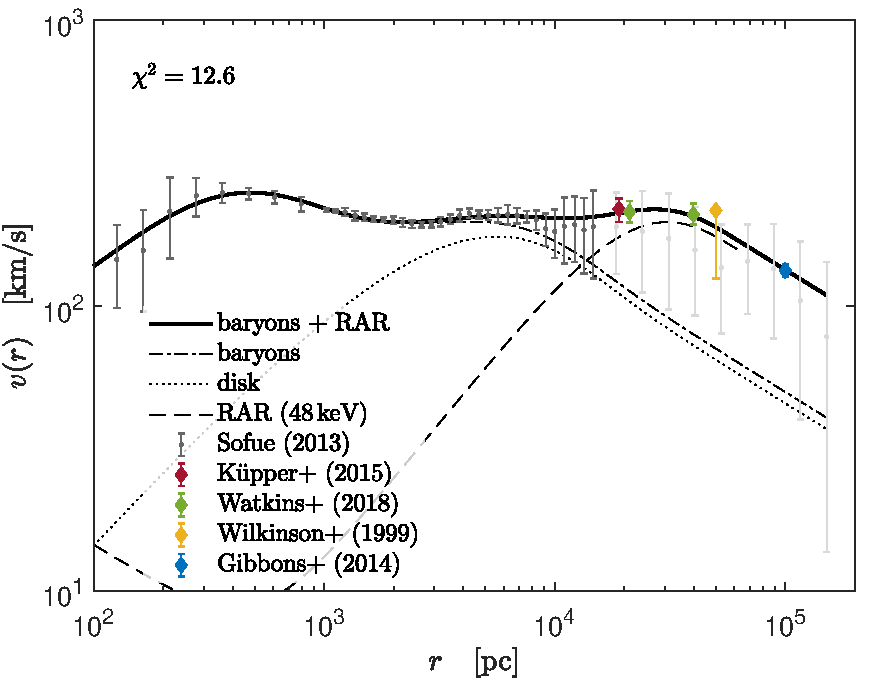
\includegraphics[width=\hsize]{\ROOTPATH/rar.pdf}
	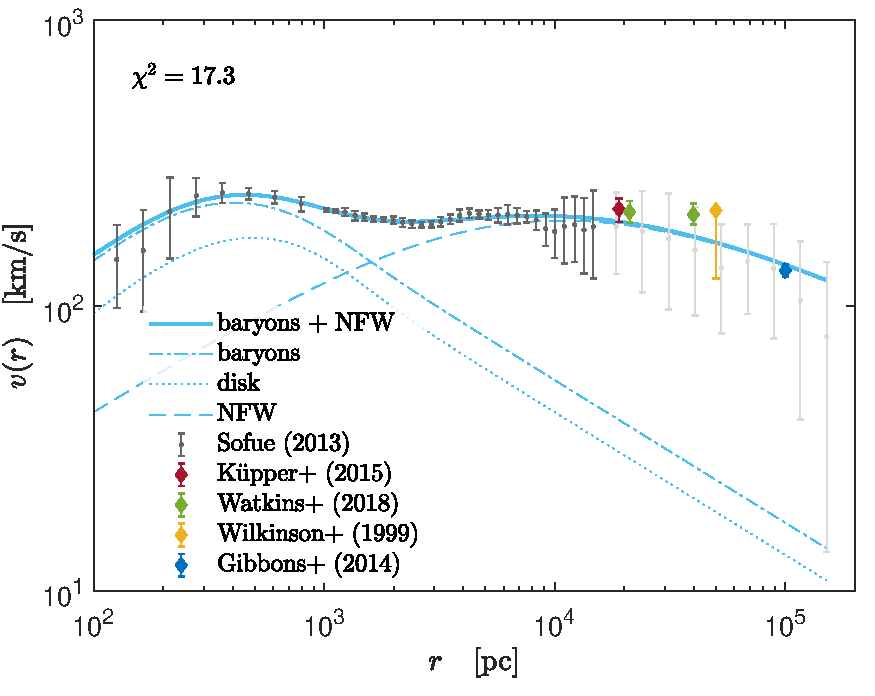
\includegraphics[width=\hsize]{\ROOTPATH/nfw.pdf}
	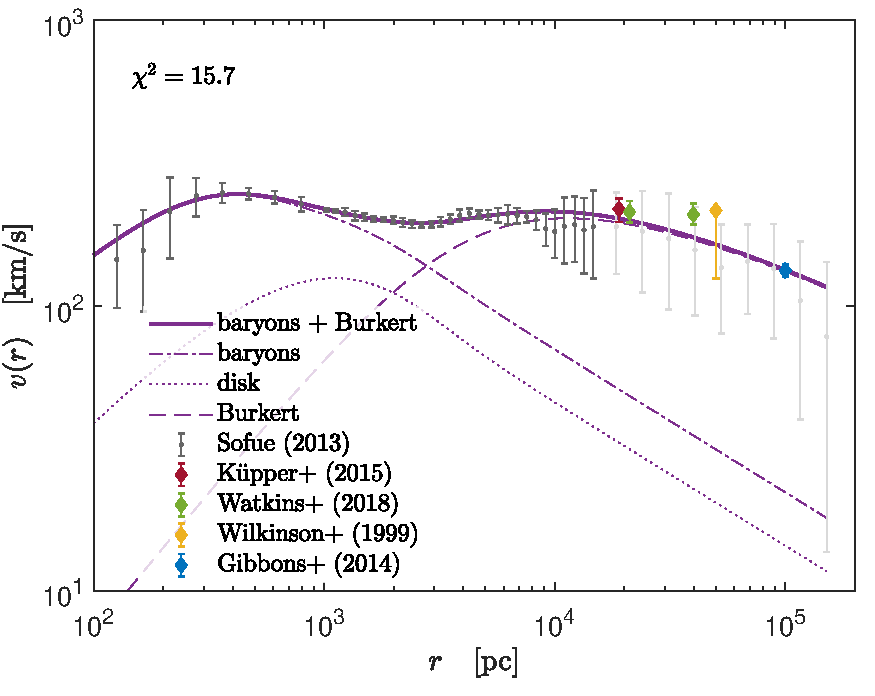
\includegraphics[width=\hsize]{\ROOTPATH/burkert.pdf}
	\caption{Rotation curve of the best-fit solution in the RAR (top), NFW (middle) and Burkert scenario (bottom).}%
	\label{fig:vrot}%
\end{figure}}
